% ICASSP 2019 - Paper on plucking position on the fretted string.
% --------------------------------------------------------------------------
\documentclass{article}
\usepackage{spconf,amsmath,graphicx,amsfonts}
\usepackage{svg}
\usepackage{cite}
\usepackage{tabularx,booktabs,colortbl}
\usepackage{hyperref}
\input macros.tex 
% ------
\title{Estimation of Guitar String, Fret and Plucking Position Using Parametric Pitch Estimation}
% ---------------
\name{Jacob~M\o ller Hjerrild and~Mads~Gr\ae sb\o ll~Christensen}%\thanks{Thanks to XYZ agency for funding.}}
\address{Audio Analysis Lab, CREATE, Aalborg University, Denmark\\
   \texttt{\{jmhh, mgc\}@create.aau.dk}}
%
\begin{document}
\ninept
\maketitle
%
%
% ---- ABSTRACT
%
%
\begin{abstract}
In this paper a fast yet effective method is proposed for analyzing guitar performances. Specifically, the activated string and fret as well as the location of the plucking event along the guitar string are extracted from guitar signal recordings. The method is based on a parametric pitch estimator and is derived from a physically meaningful model that includes inharmonicity. A maximum a posteriori classifier, which requires training data captured from only one fret per string. The classifier is tested on recordings of electric and acoustic guitar and performs well: the average absolute error of string and fret classification is $1.5\%$, while the error rate varies depending on the fret used for training. The plucking position estimator is the minimizer of the log spectral distance between the amplitudes of the observed signal and the plucking model and it is evaluated in proof-of-concept experiments that show that string, fret and plucking position combinations can be estimated accurately. Unlike the state of the art, the proposed works on very short segments (i.e., 40 ms), which makes it suitable for high-tempo and real-time applications.
\end{abstract}
%
\begin{keywords}
 Physical Modeling, Statistical Signal Processing, Machine Learning, Parametric Pitch Estimation, Music Information Retrieval\vspace{-.8mm}
\end{keywords}
%
%
% ---- INTRODUCTION
%
%
% %%%%%%%%%%%%%%%%%%%%%%%% NOTES  %%%%%%%%%%%%%%%%%
%
% why is the topic of interest ?
%
% - guitar playing style. Where does Jimi Hendrix put his fingers ?
% - Tablature
% - (in general: music transription)
% - guitar tuning
% - parametric pitch estimation
% - physical modeling.
%
% What is the background on potential solutions
%
% What was attempted in the present effort research project.
% 
% ... the simplicity of both the model, the feature set and the complexity of the algorithm a model based approach leads to an effective solution for the proposed.  
% 
% %%%%%%%%%%%%%%%%%%%%%%%%%%%%%%%%%%%%%%%%%%%%%%%
%
\section{Introduction} % (fold)
\label{sec:introduction}
\vspace{-.6mm}
%

Analysis of musical performances of individual instruments can be used for many applications, including automatic transcription and recognition of artists via analysis of stylistic details. Several papers have studied the analysis and synthesis of plucked string instruments e.g., acoustic guitar~\cite{Karjalainen93towardshigh-quality,laurson2001methods} and electric guitars~\cite{sullivan1990extending}. We are here concerned with the analysis of guitar signals. To date, there are few papers on extracting information from electric guitar recordings, some examples being work concerned with classifying the types of effects used~\cite{abesser2012feature} and estimating the decay time of electric guitar tones~\cite{pate2014predicting}. Other research involved extracting information from related string instruments, such as extracting plucking styles and dynamics for classical guitar~\cite{erkut2000extraction} and electric bass guitar~\cite{abesser:automatic_string_detection_ml}. Recent papers introduce techniques to model the physical interactions of the player with the guitar to synthesize a more realistic guitar sound, such as modeling the interactions of the guitar pick~\cite{germain2009synthesis,evangelista2010player} or fingers~\cite{poirot_nonlinear_interactions_with_string} with the string, and the fingers with the fretboard~\cite{bilbao2015numerical}.

%The motivation for this work is to understand the factors that influence the sound of well-known guitarists, in order to be able to replicate their sound by extracting the relevant parameters from their recordings. 

It is well-known that the plucking position and pickup position produce a comb-filtering effect in the spectrum of the guitar signal~\cite{fletcher:plucked_strings,fletcher:principles_of_vibration_and_sound} and that stringed instruments are not perfectly harmonic which some of the first theoretical studies on inharmonicity show~\cite{donkin:acoustics,rayleigh:sound}. Shankland and Coltman~\cite{coltShank} showed how inharmonicity is mainly caused by stiffness and deflection, which was elaborated on in~\cite{rossing:science_of_string_instruments}. The well-known piano model of inharmonicity was derived by H. Fletcher in~\cite{fletcher:piano_model} and has been used recently for string classification purposes; the inharmonicity coefficient has been proposed for electric guitar string classification contained in a 48-dimensional feature set~\cite{abesser:automatic_string_detection_ml}, where the inharmonicity coefficient was selected as one of the most discriminative features. A string and fret classification algorithm was proposed~\cite{dittmar:realtime_string_detection}, using a 10
-dimensional feature set and an SVM classifier. Large feature sets are prone to overfitting and rarely contribute to simple and meaningful findings in terms of physical cause and effect relationship. However, Barbancho et al.~\cite{barbancho:inharmonicity_tablature} proposed an inharmonicity and amplitude based method for automatic generation of guitar tablature, where they locate the fundamental frequency using heuristic for finding peaks in the spectrum. Papers that studied the estimation of the plucking event location of the guitar string have used both frequency-domain~\cite{DBLP:conf/icassp/MohamadDH17,traube:pluckin_point_dafx,traube2003extraction} and time-domain~\cite{penttinen2004time} approaches, but only for open strings or by assuming a known pitch or string and fret position. \\
%
\indent In this paper, we consider the fretted string scenario, hence the estimation of plucking event location and classification of string and fret. Thus, the objective is to extract the location of interactions of both hands of the guitar player when both hands can be arbitrarily located along a string. Generally, the left hand changes the pitch and the right hand activates the string vibration by plucking as shown in Fig.~\ref{fig:guitar_overview}. We do this using a feature set consisting of three physically meaningful parameters that are extracted with a non-linear least squares (NLS) pitch estimator~\cite{nielsen2017fast,multipitch,hansen2018parametric,DBLP:journals/sigpro/ChristensenSJJ08}, which is extended to include inharmonicity.  We use the inharmonic pitch estimates for training a Bayes maximum a posteriori (MAP) classifier of string and fret combinations which requires training data captured from only one fret on each string, such that a guitar player will be able to swiftly train his guitar on the fly.  Finally, the proposed method estimates the plucking position for the fretted string scenario, as opposed to existing work, e.g.,  \cite{traube:pluckin_point_dafx,DBLP:conf/icassp/MohamadDH17}, which was done for open strings only. All this is done on a segment-by-segment basis and using short segments.
%The method is tested on electric and acoustic guitars, recorded for this purpose. % and is available online along with MATLAB code. 
\begin{figure}[h!]\
  \centering
  \centerline{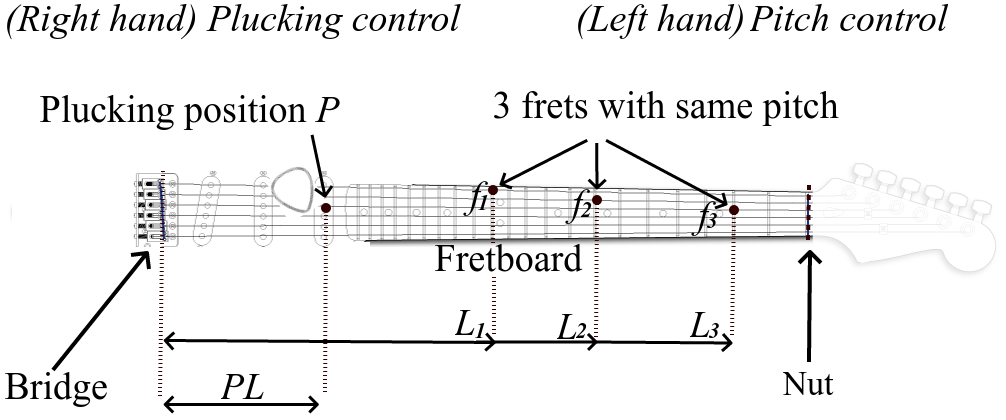
\includegraphics[width=.9\columnwidth]{img/fender_drawing7.png}}\vspace{-2mm}
  \caption{Right hand controls plucking position and left hand controls pitch using the fretboard. One pitch is produced in various positions.
  }\label{fig:guitar_overview}\vspace{-2mm}
\end{figure}


%. In the following we describe the model of the guitar string. 
% \indent The paper is structured as follows: Section~\ref{sec:signal_model} derives the inharmonic signal model for the guitar string including an ideal model of string excitation. Section~\ref{sec:proposed_method} explains a method to estimate the plucking position on the fretted string after classification of the string/fret combination based on the inharmonic pitch estimates. In Section~\ref{sec:experiments}, we evaluate the method on two data sets: (1) we evaluate the accuracy of the classifier when various frets are used for training, and (2) we evaluate the plucking
% position estimates for fretted strings given various fret and string classes. Finally, Sec.~\ref{sec:conclusion} gives the conclusion. \vspace{-.8mm}
% %
%
%
% ---- STRING AND SIGNAL MODEL
%
%
\vspace{-1.9mm}
\section{String Model} % (fold)
\label{sec:signal_model}
\vspace{-.6mm}
We start by modeling string displacement activated by plucking, before the signal parameters of interest is described. 
The vibrating part of the string has length $L$ and is fixed at $l=0$ and $l=L$ with pinned boundaries. %, hence $y(0,t)=0$ and $y(L,t)=0$. 
For a small displacement $y$, the motion is described by the partial differential equation $\frac{\partial^2 y}{\partial t^2} = c^2\frac{\partial^2 y}{\partial l^2}$, where $c$ is the speed of the transverse wave. The well-known ideal string solution is ~\cite{fletcher:principles_of_vibration_and_sound}
\begin{align}
     y(l,t) = \sum_m \big(A_m \sin{\omega_mt} + A'_m \cos{\omega_mt}\big) \sin{\kappa_ml},
\end{align}
%
where $\omega$ is frequency, $\kappa_m=\omega_m/c$ and $C_m\!\!=\!\!\sqrt{A_m^2\!+\!{A'}_m^2}$ are the wave number and the amplitude of the $m$th mode, respectively. 
%
The string is modeled with an initial deflection $\delta$ excited at plucking position $P$, by the plucking hand with an edge sharp pick at the $P$th fraction of its length ($0\!\! <\!\! PL\!\! <\!\! L$). There is no initial velocity i.e. $ \frac{\partial y}{\partial l} \!\!= \!\dot{y}(l,0)\!=0, \  \forall l$ and we assume an initial triangular string shape, i.e. 
\begin{equation}
     y(l,0) =\begin{cases}
               \frac{\delta}{P}\frac{l}{L}, \quad & 0\leq l \leq PL\\
               \frac{\delta}{1\!-\!P}(1\!-\!\frac{l}{L}),        \quad & PL\leq l \leq L. 
            \end{cases}\label{eq:string_initialization}
\end{equation}
For a fixed $P$, the $m$th Fourier coefficients of this string is 
\begin{align}
    C_m(P) \!\! &= \!\! \frac{2}{L}\bigg[\! \frac{\delta}{PL} \! \int_0^{PL}\!\!\!\!\!\!\!\!\! l \sin{\!\frac{m\pi l\!}{L}}\:\! dl\! 
        + \!\frac{\delta}{1\!-\!P}\!\!\! \int_{PL}^L \!\!\!(1\!-\!\frac{l}{L}) \sin{\! \frac{m\pi l\!}{L}}\:\! dl \bigg]\nonumber \\
        &= \frac{2\delta}{m^2 \pi^2 P(1-P)} \sin{m \pi P }, \label{eq:pluck_closed_form}
\end{align}
which explains how timbre changes as a function of plucking position. From~\eqref{eq:pluck_closed_form} it is clear that the $m$th amplitude is scaled by $m^{-2}$ with a sinusiodal spectral envelope caused by $P$, independent of pitch. From an open string length $L_{\textup{open}}$ (from bridge to nut) and a given fret $\fret_1$, the corresponding vibrating string length $L_1$ is given by $L_1 = L_{\textup{open}}  2^\frac{-\fret_1}{12}$ (see Fig.~\ref{fig:guitar_overview}).

For an electric or semi-acoustic guitar, the displacement $y(l,t)$ is measured with an electrical transducer (a pickup), which we assume is close to the vibrating string in a fixed location $(l=\lambda)$. For a discrete time sampled signal at time instance $n$ we define the signal
\begin{equation}
     x(n)  \vert_{l=\lambda} \propto y(\lambda, t),
\end{equation}   
where $x(n)$ is the guitar signal recorded with the pickup at $\lambda$. We propose to parametrize $x(n)$ with an inharmonic signal model as explained in the following. 
%
 At time instance $n$, the observed complex-valued signal vector $\vecx \in \mathbb{C}^N$ is represented as $\vecx = [x(0) \, x(1) \, \cdots \, x(N-1)]^T$, with $T$ denoting the transpose. %Do we need this?
A complex signal can ease both notation and computational complexity and a real-valued signal is converted to complex by using the Hilbert transform~\cite{LawrenceMarple1999}. The $n$th entry of $\vecx$ is modeled as an inharmonic sinusoidal part and a noise part i.e.,  
\begin{equation}\label{eq:sigmod1}
  x(n)\! =  \!\sum\limits_{m=1}^{M}\!\! \alpha_{m} \exp\big({j\psi_m(\omega_0,B) n}\big)+v(n), 
  %x(n)\! = \!s(n)\!+\!v(n)\!= \!\sum\limits_{m=1}^{M} \alpha_{m} e^{j(m\omega_0 \sqrt{1+B m^2}) n}+v(n), 
\end{equation}
where $\omega_0$ is the fundamental frequency, $M$ is the number of partials, $\alpha_{m}$ is the complex amplitude of the $m$th partial, $v(n)$ is noise and the instantaneous frequency  $\psi_m(\omega_0,B)$ is derived in~\cite{fletcher:piano_model} as
\begin{equation}
  \psi_m(\omega_0,B) = m \omega_0 \sqrt{1+B m^2}. 
\end{equation}
For ease of notation, we denote it as $\psi_m$ although it is a function of $\omega_0$ and $B$. The model order $M$ can be estimated~\cite{nielsen2017fast,multipitch}, while for the string model, initialized by the triangular shape in~\eqref{eq:string_initialization} we assume a high $M$ at the onset event. In vector-matrix notation the observed signal is modeled as
\begin{equation}\label{eq:xZa}
  \vecx = \matZ \vecalpha + \vecv,
\end{equation} 
where the complex sinusoidal matrix $\matZ \in \mathbb{C}^{N\times M}$ is given by
\begin{align}
  \matZ =& \left[ \vecz(\psi_1) \: \vecz(\psi_2) \: \cdots \: \vecz(\psi_M)\right], \\
  \vecz(\psi_m) =& \left[ 1 \: e^{j\psi_m} \: e^{j\psi_m2} \: \cdots \: e^{j\psi_m(N-1)} \right]^{T},
\end{align}
where $\vecalpha = [\alpha_1 \: \cdots \: \alpha_M]^T$ is a vector containing complex amplitudes and $\vecv = [v(0) \: v(1) \: v(N-1)]^T$ contains all noise terms. We denote the unknown and deterministic parameters with $\vectheta$, i.e.
\begin{equation}\label{eq:theta_parameters}
  \vectheta = \{\omega_0, B, \vecalpha\}.
\end{equation}
The amplitudes $\vecalpha$ can be estimated with the least squares, while the other parameters $\omega_0$ and $B$ are non-linear. 
The inharmonic pitch and inharmonicity coefficient estimates $\{\widehat\omega_0, \widehat B \} $ are sufficient for classification of string and fret~\cite{barbancho:inharmonicity_tablature,michelson2018_aes} and the estimated amplitude vector $\vecalphahat$ is used for estimation of the plucking position $\widehat{P}$.% on the vibrating string with length $\hat{L}$, implicitly given by the inverse proportionality of the pitch estimate $\omega_0$ and the full string length.
%     
%
%
% ---- PROPOSED METHOD
%
%
%
\section{Proposed Method} % (fold)
\label{sec:proposed_method}
\vspace{-.6mm}
Fig.~\ref{fig:overview} gives an overview of the proposed method. The proposed method is initialized with a detection of the onset event from which one segment is extracted and the following estimation is done on such a segment alone. The feature set in~\eqref{eq:theta_parameters} is extracted as maximum likelihood with the NLS inharmonic pitch estimation method. $\{\widehat\omega_0, \widehat B \} $ are applied to a MAP classifier of string and fret. At the estimated inharmonic frequencies $\widehat{\boldsymbol{\psi}}$, the complex amplitudes $\vecalphahat$ are estimated using least squares. These are used for estimation of plucking position $\widehat{P}$. All details are derived in the following.
In this study the onset detection is considered a solved problem which can be obtained with a filter bank method~\cite{olivier:mirtoolbox_dafx}.% command $\texttt{mironsets(x,'filter','diff','contrast',0.2)}$.
%
%
% ---- PITCH ESTIMATION (Proposed method)
%
%
\subsection{Inharmonic Pitch Estimation} % (fold)
\label{sec:proposed_estimator}
\begin{figure}[t]\
  \centering
  \centerline{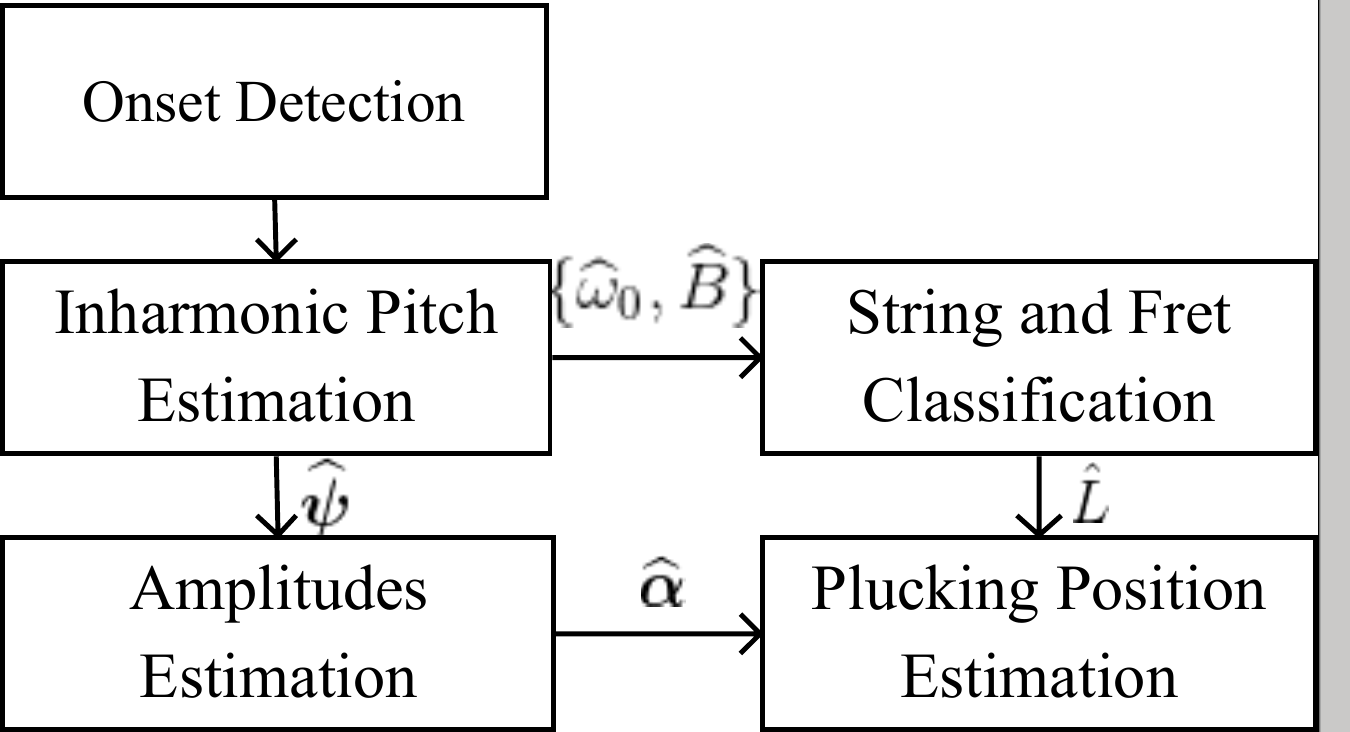
\includegraphics[width=.75\columnwidth]{img/block2.png}}\vspace{-2mm}
  \caption{Overview of the proposed method.}\label{fig:overview}\vspace{-2mm}
\end{figure}
The pitch and inharmonicity parameters are estimated by maximizing the likelihood function %probability of the observed data $\vecx$ given the parameters:
\begin{equation}
    \thetahat = \argmax{\vectheta}{\Like(\vectheta | \vecx)} = \argmax{\vectheta}{p(\vecx ; \vectheta)}.
\end{equation}
The observed signal distribution is modeled in circular complex white Gaussian noise with covariance matrix $\C$, i.e., 
\begin{equation} 
    p(\vecx ; \vectheta) = \frac{1}{\pi^N\det{(\C)}} e^{\left(-\vecv^H\C^{-1}\vecv\right)},
\end{equation}
where $\C=\sigma^2\I$ is a diagonal matrix, scaled by an unknown variance $\sigma^2$, where $\I$ is the $N \times N$ identity. By the use of~\eqref{eq:xZa} with $\vecv = \vecx - \matZ \vecalpha$, 
the log-likelihood function is expressed as
\begin{equation}\label{eq:log_likelihood2}
    \ln\Like(\vectheta|\vecx) = -N \ln(\pi) - N \ln \frac{1}{N}|| \vecx-\Z \vecalpha ||_2^2 - N.
\end{equation}
By neglecting all terms that do not dependent on $\omega_0$ and $B$, the maximum likelihood solution is the minimizer of the 2-norm error between the observed signal and the signal model, expressed as
\begin{equation}
  \thetahat =  \argmax{\vectheta}{\Like(\vectheta | \vecx)}  =\argmin{\vectheta}{\norm{\vecx-\Z \vecalpha}_2^2}.
\end{equation}
By substituting $\vecalpha$ with its least squares estimate
\begin{equation}\label{eq:alphahat}
  \vecalphahat = (\Z^H\Z)^{-1}\Z^H\vecx,
\end{equation}
the inharmonic non-linear least squares (NLS) pitch estimator is
\begin{equation}\label{eq:psi_B_est}
  \{ \widehat\omega_0, \widehat B \}= \argmin{\psi_0, B}{|| \vecx - \Z(\Z^H\Z)^{-1}\Z^H\vecx}||_2^2.
\end{equation}
Asymptotically $N(\Z^H\Z)^{-1}\!\!=\!\I|_{N\to\infty}$ , a computationally efficient approach can be found as
\begin{equation} \label{eq:ANLS}
    \{\widehat\omega_0, \widehat B \} = \argmax{\psi_0,B}{\vecx^H \matZ \matZ^H \vecx} = \argmax{\psi_0,B}{ \norm{\matZ^H\vecx}_2^2},
\end{equation}
which can be implemented using just one FFT per segment. Since $B\!<\!<\!1$, an initial pitch estimate is obtained with $B=0$, and from that we define a narrow two dimensional search grid for the inharmonic pitch ($\omega_0$ and $B$) to ease computational complexity. An optimal grid can be selected using~\cite{jkn:grid_size}. Finally, the amplitudes are estimated using~\eqref{eq:alphahat}.
%
%
%
% ---- CLASSIFICATION (Proposed method)
%
%
%
\subsection{String and Fret Classification} % (fold)
\label{sec:proposed_classification_of_string_and_fret}
Having found the pitch and the inharmonicity parameters $\vecphi = [\widehat\omega_0, \widehat B ]^T$ using~\eqref{eq:ANLS}, the next problem is to classify the observed signal $\vecx$ as being produced by a string and fret position. We have a set of $K$ mutually exclusive classes $\symvec{\Gamma}=\{\gamma_1,\dots,\gamma_K\}$ representing all possible string and fret positions. The MAP-optimal classifier with decision function $\hat{\gamma}(\cdot)\!:\! \mathbb{R}^I \!\!\!\rightarrow \!\!\boldsymbol{\Gamma}  $ is~\cite{mspr}
\begin{align}
    \hat\gamma_{\textup{MAP}}(\vecphi) &= \argmax{\gamma\in\Gamma}{p(\gamma|\vecphi)} = \argmax{\gamma\in\Gamma}{p(\vecphi|\gamma)P(\gamma)}.
\end{align}
We model $\vecphi$ as coming from a normal object with class $\gamma_k$, then the $k$th conditional probability density is   
\begin{equation}
    p(\!\gamma_k\lvert\vecphi)\! = \!\! {{(\!2\pi\!)^{\!\!-1}\!\!\det{\!(\!\boldsymbol{\Lambda}_k\!)\!^{\!\frac{\!-\!1}{2}}\!\!}}}\, \exp\!\!\bigg(\!\!\frac{-(\!\vecphi-\boldsymbol{\mu}_k\!)^T\!\boldsymbol{\Lambda}_k^{-1} (\!\vecphi-\boldsymbol{\mu}_k\!) }{2}\!\! \bigg),
\end{equation}
where the expectation vector $\boldsymbol{\mu}_k$ and covariance matrix $\boldsymbol{\Lambda}_k$ are given from training. The covariance matrix is here modeled as being class independent and isotropic, i.e., we have that $\boldsymbol{\Lambda}_k=\sigma^2\mathbf{I}$. There are several reasons for this. First, as we shall see, it proves sufficient for very accurate classification. Second, it requires very little training data, something that is important due to the high number of classes formed by combinations of strings and frets. We also remark that using a simple statistical model is also desirable in that it makes it possible to adapt the classifier to specific instruments using a simple training procedure. Returning now to the classifier, neglecting terms that do not depend on the class index $k$ yields the following, simple classification scheme:
\begin{equation}\label{eq:classifier}
  \hat{\gamma}(\vecphi)\!\!=\!{\gamma}_i \;\; \textup{with} \;\; 
  i\!=\!\argmax{k=1,\dots,K}
  {\bigg\{\!
   2\ln\! P(\!\gamma_k)\! -\! \frac{\norm{\vecphi-\!\boldsymbol{\mu}_k}^2}{\sigma^2}\! \bigg\}}\!.
\end{equation}
As can be seen, the classifier in~\eqref{eq:classifier} is the minimizer of the Euclidean distance between the observation and its expectation, with a correction factor of $2\sigma^2 P(\gamma_k)$. The prior $P(\gamma_k)$ can be specified from the number of training samples from class $\gamma_k$ or be assumed uniform, in which case it reduces to a maximum likelihood classifier. 
% For Euclidean distance, we normalize both features to have an absolute maximum of 1.
%
%
%
% ---- TRAINING (Proposed method)
%
%
%
%\subsubsection{Training Procedure} % (fold)
%\label{ssub:fast_training}

The model parameters of each class $\{\boldsymbol{\mu}_k, \boldsymbol{\Lambda}_k\}, \forall k$, can be found from a labelled set of $I$ i.i.d. samples $\{\vecphi\}$. % where $\vecphi^{(i)}$ is the $i$th estimate $\{\widehat\psi_0^{(i)}, \widehat B^{(i)} \}$ from~\eqref{eq:ANLS}. 
However, it is in fact possible to obtain a model for all frets on a string from one such model. For example, given the parameters $B_s( \fret_1 )$ and $\omega_{0,s}( \fret_1 )$ of the $s$th vibrating string for a given fret $\fret_1$, the corresponding parameter can be computed for any other fret $\fret_2$, using the inharmonicity model derived in~\cite{barbancho:inharmonicity_tablature}
\begin{equation}\label{eq:B_definition}
    \widehat{B}_s( \fret_2 ) =  \widehat{B}_s( \fret_1 ) \: 2^{ \frac{  \fret_2 - \fret_1 }{ 6 }} = \frac{ \pi^3 E_s d_s^4 }{ 64 T_s L^2_{s}(\fret_2) },
\end{equation}
and for the pitch estimates we have that
%\begin{equation}\label{eq:omega0_fast}
  $\widehat{\omega}_{0,s}( \fret_2 ) =  \widehat{\omega}_{0,s}( \fret_1 ) 2^{\frac{\fret_2-\fret_1}{12}}$.
%\end{equation}
Hence, the classifier only need to be trained using audio captured from one fret per string in order to model the parameters of the remaining frets. In~\eqref{eq:B_definition} $E_s$ is elastic modulus, $d_s$ is core diameter, $T_s$ is tension, which can be considered constants~\cite{rossing:science_of_string_instruments}. %Aside from lowering the computational complexity,~\eqref{eq:B_definition} and~\eqref{eq:omega0_fast} are used in a $13$-fold hold out scheme where one model is trained on data one fret and classify the remaining data 12 frets. 
\vspace{-.8mm}
\subsection{Plucking Position Estimation} % (fold)
\label{sec:proposed_estimation_of_pluck_amplitude}
\vspace{-.6mm}
As was argued earlier, once the estimate of amplitudes has been obtained using~\eqref{eq:alphahat}, the plucking position $\widehat{P}$ can be found. More specifically, the plucking position, $\widehat{P}$, is found in the proposed method by minimizing the log spectral (LS) distance between the observation $\vecalphahat$ and the model $\mathbf{C}$, i.e., 
\begin{equation}
    \widehat{P} = \argmin{P}{\big(d_{\textup{LS}}(\vecalphahat,\mathbf{C}(P))\big)},
\end{equation}
where $\mathbf{C}(P) = [C_1(P),C_2(P),\dots,C_M(P)]^T$ is obtained from the model in~\eqref{eq:pluck_closed_form} and the log spectral distortion is defined as
\begin{equation}
    d_{\textup{LS}}(\vecalphahat,\mathbf{C}(P)) = \sqrt{ \frac{1}{M} \sum_m 10\log_{10} \frac{\lvert\widehat{\alpha}_m\rvert^2}{\lvert C_m(P)\rvert^2} }.
\end{equation} 
We remark that the model $\mathbf{C}$ can be even more physical meaningful by combining it with a model of the pickup location, such as the model in~\cite{DBLP:conf/icassp/MohamadDH17}.\vspace{-2mm}
%
%
% ---- EVALUATION 
%
%

\begin{table}\centering %\vspace{-1mm}
\caption{String and fret confusion matrix for the Martin  acoustic guitar. The classification errors are shown for each of the 6 strings.}
\label{tbl:string_confusion_martin}
\begin{tabularx}{0.46\textwidth}{@{}l*{7}{c}c@{}}
\toprule
Labels &Est. 6   &Est. 5 &Est. 4   &Est. 3   &Est. 2   &Est. 1   \\ 
\midrule
True 6   &1560 \cellcolor[gray]{.8} &0  &0  &0  &0  &0  \\  
True 5   &0  & 1560\cellcolor[gray]{.8} & 0   &0  &0  &0  \\
True 4   &0  &0  &1560 \cellcolor[gray]{.8} &0  &0  &0  \\  
True 3   &0  &0  &0  &1560 \cellcolor[gray]{.8} &0  &0  \\  
True 2   &0  &0  &0  &0  &1560 \cellcolor[gray]{.8} &0  \\  
True 1   &0  &0  &0  &0  &0  &1560 \cellcolor[gray]{.8} \\  
\bottomrule
\end{tabularx}
%\end{table}%\vspace{-.6mm}
%
%\begin{table}%\centering \vspace{-.6mm}
\caption{String and fret confusion matrix for the Firebrand electric guitar. The classification errors are shown for each of the 6 strings}
\label{tbl:str_confusion_firebrand}
\begin{tabularx}{0.46\textwidth}{@{}l*{7}{c}c@{}}
\toprule
Labels &Est. 6   &Est. 5 &Est. 4   &Est. 3   &Est. 2   &Est. 1   \\ 
\midrule
True 6   &1536 \cellcolor[gray]{.8}       & 24                        &0      &0  &0  &0 \\
True 5   &0  & 1560\cellcolor[gray]{.8}   & 0                        &0      &0  &0  \\
True 4   &0  &0  &1475 \cellcolor[gray]{.8}                           & 85   &0  &0  \\
True 3   &0  &0  &76                     &1455 \cellcolor[gray]{.8}   & 29   &0  \\
True 2   &0  &0  &0  &0                   &1506 \cellcolor[gray]{.8}  & 54  \\
True 1   &0  &0  &0  &0                   &0                          &1560 \cellcolor[gray]{.8} \\
\bottomrule % \vspace{-6mm}
\end{tabularx}
\end{table}
\section{Evaluation} % (fold)
\label{sec:experiments}
%\vspace{-.6mm}
To evaluate the proposed plucking position estimator along with the string and fret classifier, some experiments have been conducted as described next. These experiments focus on segment-by-segment estimation and classification using short segments, as this enables high-tempo and real-time applications of the proposed method. Hence, the experiments aim to demonstrate that this is possible. In relation to this, we remark that the state of the art \cite{barbancho:inharmonicity_tablature,michelson2018_aes} operates on multiple segments, each in the order of 100 ms. As the NLS estimator has been shown to reach the Cram{\'e}r-Rao lower bound~\cite{nielsen2017fast}, we do not go into further details about this. The proposed method was evaluated on recorded data (44.1 kHz). The data and MATLAB code is available online\footnote{\url{https://tinyurl.com/yc76blld}}. The data consists of guitar recordings of the electric and acoustic guitar, each labelled with their respective string and fret combination, namely electric Les Paul Firebrand with Elixir Nanoweb (.10-.54) strings and an acoustic Martin DR with SP (.12-.52) strings. The recorded data of each guitar represents 10 line signal recordings of every string and fret combination from the $0$th to $12$th, hence it consists of 10 recordings of 13 frets and 6 strings which resembles 720 recordings. For experiments, every recording is segmented from the detected onset time event in to a 40 ms segment. %\vspace{-.6mm}
%
%
%
%
%%%%%%%%%%%%%%%%%%%%%%%%%%%%%%%%%%%%%%%%%%%%%%%%%%%%%%%%%%%%%%%%%%%%%%%%%%%%%%%
%
% TEST SETUP TABLE
%
% \begin{table}\centering
% \caption{\label{tbl:experiments}Test setup.}
% \begin{tabularx}{0.4\textwidth}{@{}l*{7}{c}c@{}}
% \toprule
% % General Test Setup  &    \\
% % \midrule
% Sampling rate ($f_s$)  	& 44.1 kHz  \\
% Signal segment duration       	& 40 ms.  \\
% $\textbf{Guitars:}$				& \\
% Martin DRS2 &  with SP	(.12--.52) strings		\\
% Les Paul Firebrand		& with Elixir (.10--.54) strings\\
% \bottomrule
% \end{tabularx}
% \end{table}\vspace{-4mm}
%    
% \subsection{Pitch and Inharmonicity Estimation} % (fold)
% \label{sec:clustermodel_selection}
% Insert graph of inharmonicity estimation from one fret.
% %
% \subsection{String Estimation} % (fold)
% \label{sec:string_estimation}
% Insert overall average performance for both guitars. (in a table)
%%%%%%%%%%%%%%%%%%%%%%%%%%%%%%%%%%%%%%%%%%%%%%%%%%%%%%%%%%%%%%%%%%%%%%%%%%%%%%%%
%
%
% --------- EVALUATION OF CLASSIFIER
%
%
%\subsection{Classification of String and Fret} % (fold)
\label{sec:string_fret_classification}
%\vspace{-.6mm}
The classification of the string and fret is tested on recordings of both guitars. 
%~\eqref{eq:B_definition} and~\eqref{eq:omega0_fast} are used in a $13$-fold hold out scheme where one model is trained on data one fret and classify the remaining data 12 frets.
The classifier is trained as described in \ref{sec:proposed_classification_of_string_and_fret} iteratively, such that $13\times12\times6 = 9360$ recordings are classified in total. The resulting confusion matrices in Table.~\ref{tbl:string_confusion_martin} and Table.~\ref{tbl:str_confusion_firebrand} are shown here for the strings, and we observe that the acoustic guitar has a very low error rate while for the electric guitar it is on average $3\%$. The biggest confusion occurs between strings 3 and 4. We have observed that the amplitudes for $m\gg1$ of the acoustic guitar has relatively more energy than the electric guitar, which is related to string material, acoustic qualities and the electrical systems~\cite{fletcher:physics_of_musical_instruments}.  
The errors for the electric guitar are explored in Fig.~\ref{fig:err_vs_frets}. The lowest error rate would be $1\%$ from the $12$th fret, while it is $5\%$ from training in the $8$th fret. %\vspace{-.6mm}
%

%
\begin{figure}[t]
  \centering
  \centerline{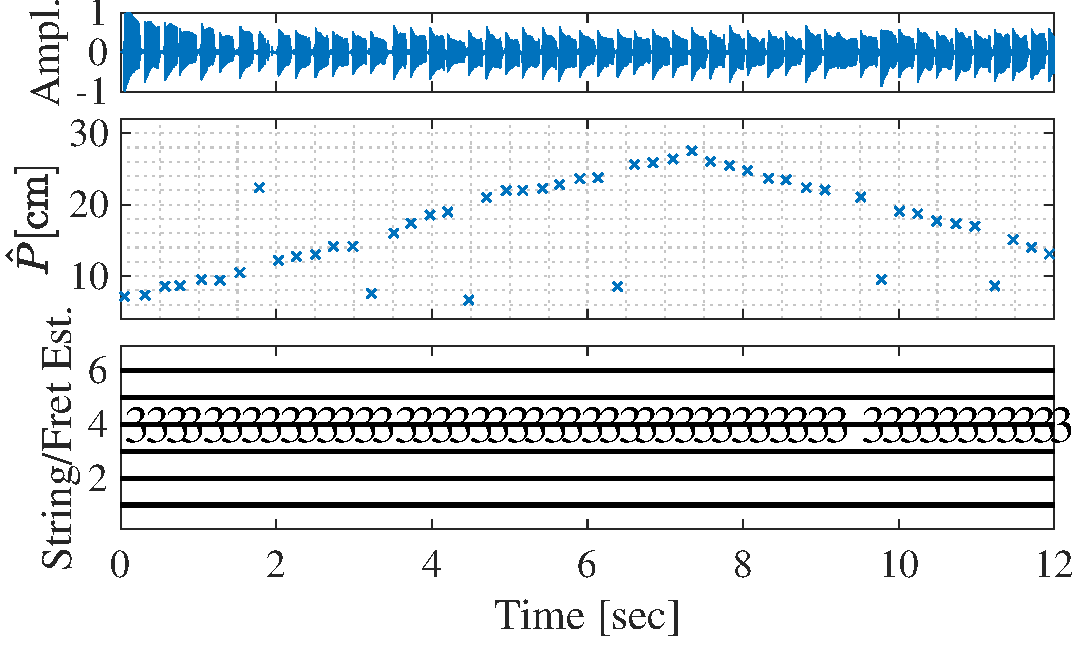
\includegraphics[width=.9\columnwidth]{img/tablature_constant_note8}}\vspace{-2mm}
  \caption{String, fret and plucking position estimates with moving plucking position and fixed string/fret for electric guitar.}\label{fig:pluck_position_fixed_tabs}
%\vspace{-.6mm}
\end{figure}%\vspace{-.6mm}
%
\begin{figure}[t]
  \centering
  \centerline{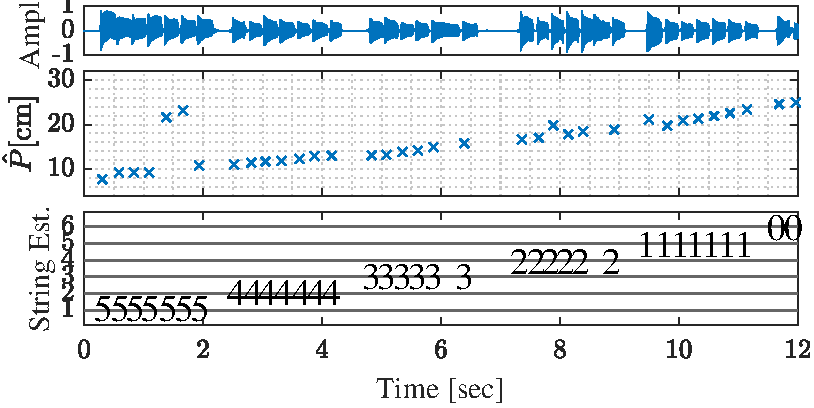
\includegraphics[width=.92\columnwidth]{img/tablature_constant_note23_LSD}}%\vspace{-2mm}
  \caption{String, fret and plucking position estimates with moving plucking position and moving string and fret for electric guitar.}\label{fig:pluck_position_varied_tabs}\vspace{-.6mm}
\end{figure} \vspace{-.8mm}
%
%\vspace{-.6mm}
\begin{figure}[htbp]
  \centering %\vspace{-6mm}
  \centerline{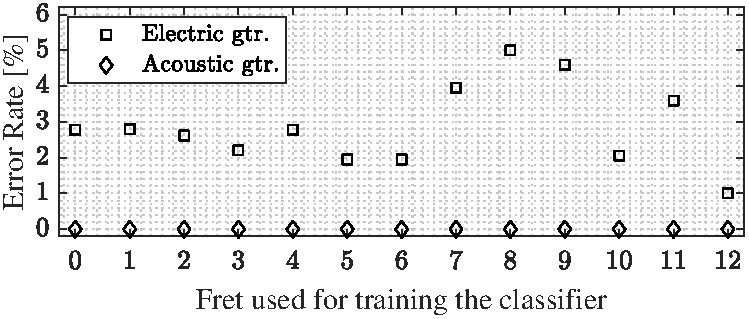
\includegraphics[width=.8\columnwidth]{img/errorRate_vs_frets2.pdf}}%\vspace{-2mm}
  \caption{String and fret classification error rate.}\label{fig:err_vs_frets}
\end{figure}%
%
%
% ----- EVALUATION OF PLUCKING ON FRETTED STRING
%
%
%\subsection{Plucking Position Estimation} % (fold)
%\label{sec:string_estimation}
Finally, the estimation of plucking position is tested on two 12 second recordings of electric guitar that resembles realistic playing with both hands continuously during each recording. Since the ground truth of plucking position is demanding to obtain, the experimental ground truth is based on a continuously moving the plucking event location; monotonously moving it from the bridge and towards the nut of the guitar. The result in Fig.~\ref{fig:pluck_position_varied_tabs} represents a case where 6 strings are being played in six frets in a structured manner. All the string and fret combinations was correctly extracted, except from one missing at the given onset events and the plucking position estimates shows a clear trend that follows the ground truth direction. In Fig.~\ref{fig:pluck_position_fixed_tabs} similar results are shown for a fixed string and fret combination, where we can observe a clear trend in plucking position direction and it is interesting that spatial aliasing occurs from 7 seconds and on-wards. %\vspace{-.6mm}
%
%
%
% ---- CONCLUSION
%
%
%
\section{Conclusion} 
\label{sec:conclusion}
%\vspace{-.6mm}
In this paper a fast method for estimation of guitar string, fret and plucking position was proposed. The proposed method works on very short guitar recording segments (i.e., 40 ms), which makes it suitable for high-tempo and real-time applications. The method is based on a parametric pitch estimator which includes inharmonicity, which effectively estimates the parameters of interest, as shown through the evaluation on both electric and acoustic guitar recordings.
%
%In this paper a fast method was proposed for estimating the plucking position which includes estimation of the activated string and fret from short segments of audio. 
The plucking position estimator is the minimizer of the log spectral distance between the estimated amplitudes of the observed signal and the plucking model; it is evaluated in proof-of-concept experiments that show that
string, fret and plucking position combinations can be estimated accurately.
%where a clear trend was demonstrated for correct plucking position as well as string and fret combinations. The feature set of the classifier is directly based on non linear least squares pitch estimation, extended to include inharmonicity; derived from a physically meaningful model. 
The MAP string and fret classifier requires training data captured from one fret per string and tested on the remaining recordings, iteratively. It was tested for all frets and yields accurate results with an overall average error rate of $1.5\%$, while the error rate varies depending on the fret used for training. The proposed method is derived from a physically meaningful model and reliably extracts the parameters that represents string, fret and plucking positions on short segments. For future work, it will be interesting to include pickup location in the model and the properties of the strings such as core and wrapping material and dimensions, could be basis for training the classifier.
%
%In this paper a fast yet effective method is proposed for analyzing guitar performances. Specifically, the activated string and fret as well as the location of the plucking event along the guitar string are extracted from guitar signal recordings. The method is based on a parametric pitch estimator and is derived from a physically meaningful model that includes inharmonicity. A maximum a posteriori classifier, which requires training data captured from only one fret per string. The classifier is tested on recordings of electric and acoustic guitar and performs well: the average absolute error of string and fret classification is $1.5\%$, while the error rate varies depending on the fret used for training. The plucking position estimator is the minimizer of the log spectral distance between the amplitudes of the observed signal and the plucking model and it is evaluated in proof-of-concept experiments that show that string, fret and plucking position combinations can be estimated accurately. Unlike the state of the art, the proposed works on very short segments (i.e., 40 ms), which makes it suitable for high-tempo and real-time applications.
%
%
% ---- BIBLIOGRAPHY
%
%
\vfill\pagebreak
\bibliographystyle{IEEEtran}
%
\bibliography{myabbr,refs}
\end{document}
%
%
% ---- SOME MORE EXPERIMENTAL RESULTS
%
%
% \begin{figure}[t]\label{fig:inharmonicity1}
%   \centering
%   \centerline{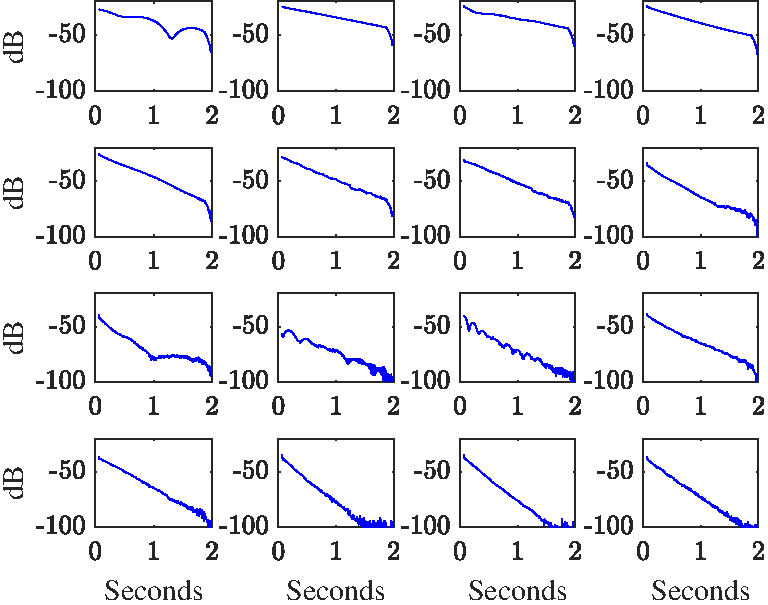
\includegraphics[width=\columnwidth]{img/spectral_decay_EString_349_long_file_partial_amplitudes}}
%   \caption{Decay of each estimated amplitude.}
% \end{figure}
% \begin{figure}[t]\label{fig:inharmonicity1}
%   \centering
%   \centerline{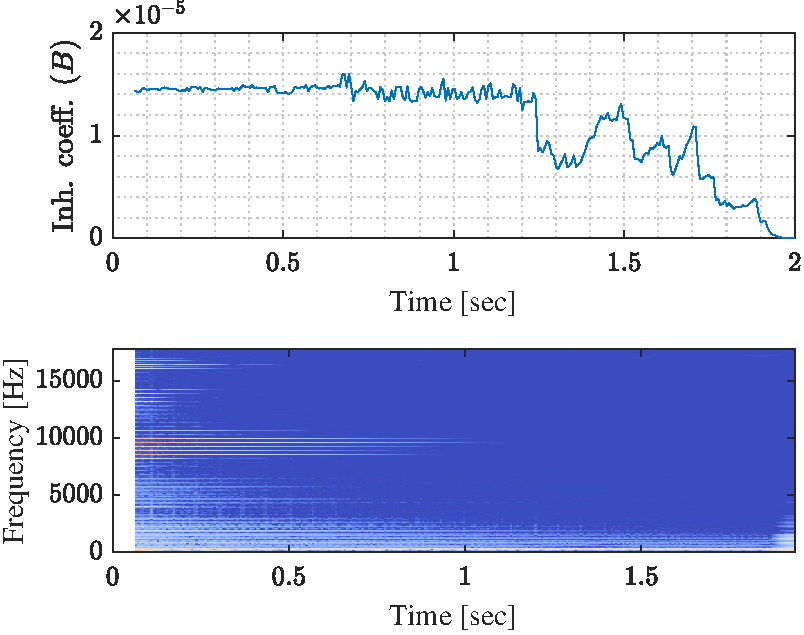
\includegraphics[width=\columnwidth]{img/spectral_decay_EString_349_long_file_inh_coff}}
%   \caption{Inharmonicity Estimates over time.}
% \end{figure}
%
%
% \begin{figure}[t]\label{fig:err_vs_frets}
%   \centering
%   \centerline{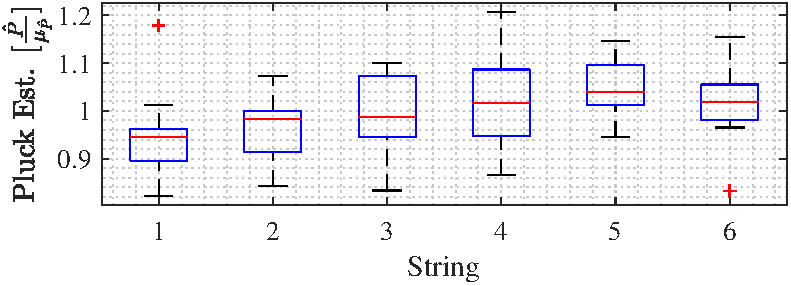
\includegraphics[width=\columnwidth]{img/pluck_est_stats_strings}}
%   \caption{Plucking position estimates normalized by their estimated mean for each string for the Firebrand electric.}
% \end{figure}
% \begin{figure}[t]\label{fig:err_vs_frets}
%   \centering
%   \centerline{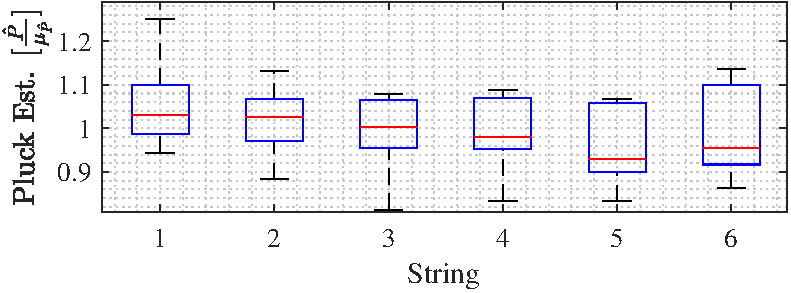
\includegraphics[width=\columnwidth]{img/pluck_est_stats_strings_martin}}
%   \caption{Plucking position estimates normalized by their estimated mean for each string for the Martin acoustic guitar.}
% \end{figure}
%\tabularnewline
%
%
%
% \begin{figure}[t]\label{fig:spectral_decay}
%   \centering
%   \centerline{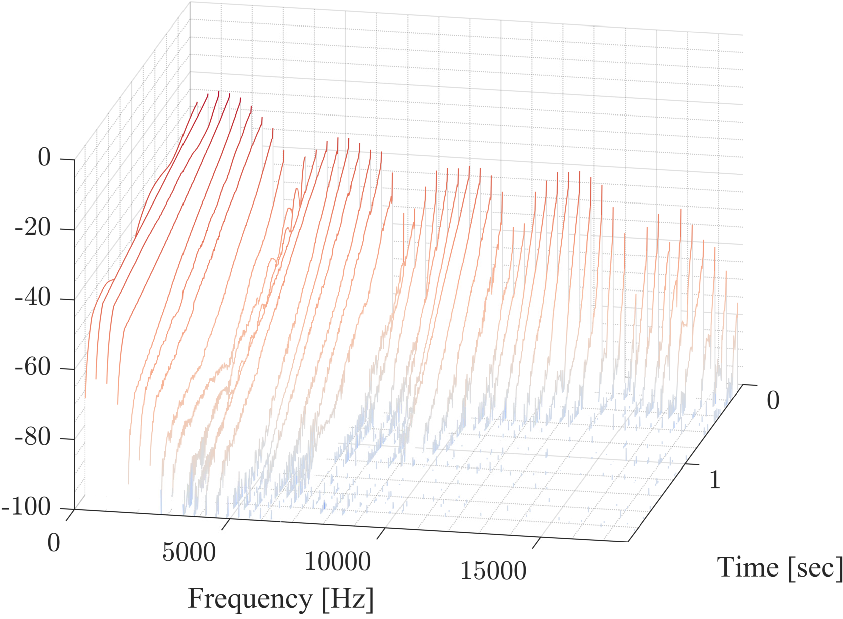
\includegraphics[width=\columnwidth]{img/spectral_decay_EString_349_long_file4}}
%   \caption{Power of the estimated amplitudes, estimated with the proposed method from a short time Fourier transform (STFT) on a plucked string on the Martin acoustic guitar. (showed in dB).}
% \end{figure}\vspace{-.6mm}%